% % % % % % % % % % % % % % % % % % % % % % % % % % % % % % % % % %
%  Devolutiva — Fase 1: Imersão
%  Disciplina: Design Thinking (DE_233) — ETE Cícero Dias
%  Profa. Samara Silva  ·  Recife, 28 de junho de 2026
% % % % % % % % % % % % % % % % % % % % % % % % % % % % % % % % % %

\documentclass[
  sigconf,
  nonacm, % Remove o rodapé da ACM
  language=portuguese
]{acmart}

% ── Desliga rodapé ACM ──────────────────────────────────────
\settopmatter{printacmref=false}
\setcopyright{none}
\acmYear{2026}
\let\balance\relax

% ── Mata a página temporária da ACM (compilação única via API) ──
\makeatletter
\def\acm@addtemp@page{}
\makeatother

% ── Pacotes ─────────────────────────────────────────────────
\usepackage[portuguese]{babel}
\usepackage{microtype}
\usepackage{booktabs}
\usepackage{tabularx}
\usepackage{array}
\usepackage{colortbl}
\usepackage[dvipsnames,table]{xcolor}
\usepackage[inline]{enumitem}
\usepackage{graphicx}
\usepackage{adjustbox}
\usepackage{fancyhdr}
\usepackage{eso-pic} % Para a capa preencher toda a página sem gerar páginas em branco

% ── Ajuste contra quebras de texto ruins (Textos Cortados) ──
\tolerance=1000
\emergencystretch=1.5em

% ── Cores ───────────────────────────────────────────────────
\definecolor{cgood}{HTML}{1E6B3A}
\definecolor{cwarn}{HTML}{8B4500}
\definecolor{cred}{HTML}{C0392B}
\definecolor{cmuted}{HTML}{666666}
\definecolor{crow}{HTML}{F2EFEB}

% ── Colunas customizadas para tabela ────────────────────────
\newcolumntype{L}[1]{>{\raggedright\arraybackslash}p{#1}}
\newcolumntype{C}[1]{>{\centering\arraybackslash}p{#1}}

% ── Comando nota destacada ───────────────────────────────────
\newcommand{\notadestaque}[2]{%
  \noindent\textbf{Nota:}\enspace%
  {\large\bfseries\color{cred}#1\,/\,#2\,pts}%
}

% ── Comando label de status ──────────────────────────────────
\newcommand{\statusok}[1]{{\small\bfseries\color{cgood}#1}}
\newcommand{\statuswarn}[1]{{\small\bfseries\color{cwarn}#1}}

% ── Renomeações PT-BR ────────────────────────────────────────
\AtBeginDocument{%
  \renewcommand{\abstractname}{Resumo}
  \renewcommand{\figurename}{Figura}
  \renewcommand{\tablename}{Tabela}
}

% ────────────────────────────────────────────────────────────
\begin{document}

% ── CAPA ────────────────────────────────────────────────────
\thispagestyle{empty}
\AddToShipoutPictureBG*{%
  \AtPageLowerLeft{%
    \IfFileExists{capa.png}{%
      
\includegraphics[width=\paperwidth,height=\paperheight]{capa.png}%
    }{%
      \IfFileExists{../../capa.png}{%
        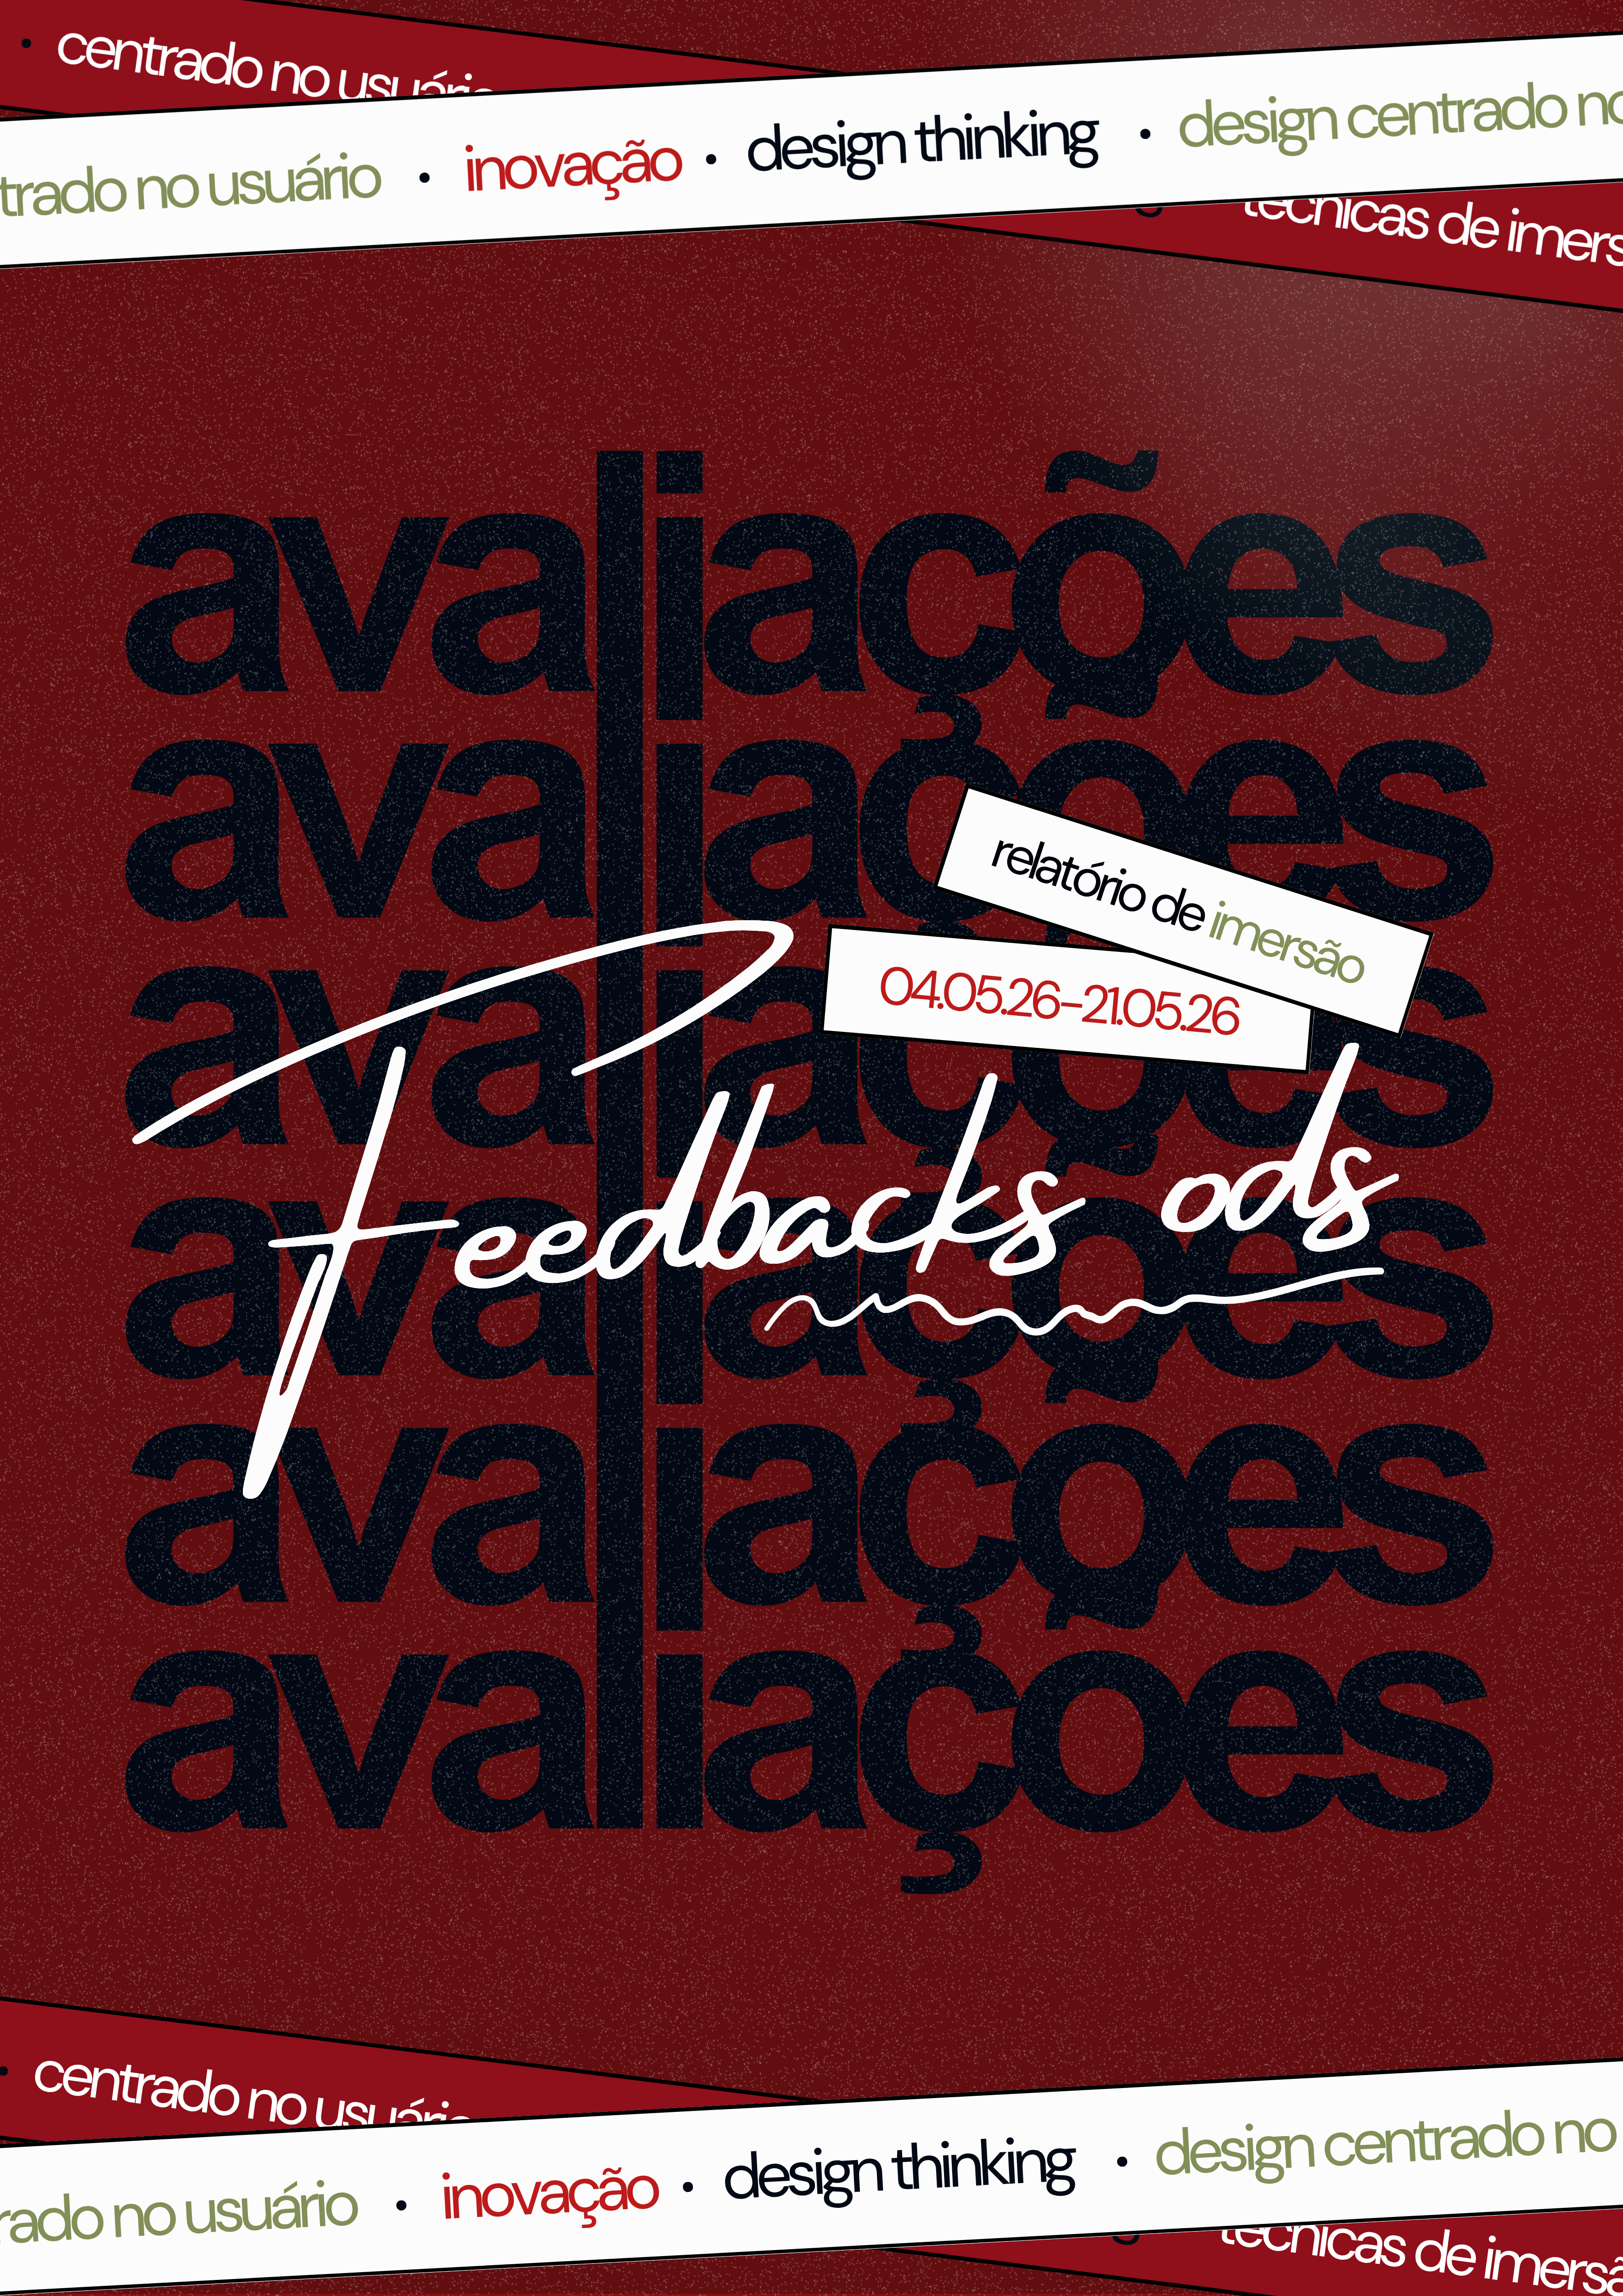
\includegraphics[width=\paperwidth,height=\paperheight]{../../capa.png}%
      }{%
        \parbox[b][\paperheight]{\paperwidth}{%
          \vspace*{10cm}\begin{center}{\large\color{gray}[capa.png não encontrada]}\end{center}%
        }%
      }%
    }%
  }%
}
\mbox{} % Caixa vazia para garantir que a página da capa seja gerada e preenchida
\clearpage

% ── CONFIGURAÇÃO DE PÁGINA PÓS-CAPA ─────────────────────────
\setcounter{page}{1}
\pagestyle{fancy}
\fancyhf{}
\renewcommand{\headrulewidth}{0pt}
\fancyfoot[C]{\thepage}
\setlength{\headsep}{0.8cm} % Distancia o cabeçalho do conteúdo das colunas

% ── METADADOS ────────────────────────────────────────────────
\title{Feedback Avaliativo de Projeto: Design Thinking --- Avaliação Completa}

\author{Profa.\ Samara Silva}
\authornote{Grupo: \textbf{Grupo 06 - Alfabetização} \textperiodcentered\ Per\'{i}odo: 22 de maio de 2026 \textperiodcentered\ Avaliado em: 28 de junho de 2026.}
\email{samarasilvia.educa@gmail.com}
\affiliation{%
  \institution{ETE C\'{i}cero Dias}
  \department{M\'{o}dulo 1 --- Turma A · 2026.1}
  \city{Recife}
  \state{Pernambuco}
  \country{Brasil}
}

\author{Grupo 06 - Alfabetização}
\affiliation{%
  \institution{ETE C\'{i}cero Dias}
  \department{Turma --- Turma A · 2026.1}
  \city{Recife}
  \state{Pernambuco}
  \country{Brasil}
}
\maketitle

\vspace{1em}
\section{Avaliação — Design Thinking}

\notadestaque{9,27}{11,00}

A seguir o detalhamento por fase da disciplina.

\subsection{Fase 1 — Imersão}

\notadestaque{2,92}{3,00}

\subsubsection*{Resumo dos Critérios}

\rowcolors{2}{crow}{white}
\begin{tabular}{@{} L{2.6cm} C{2.5cm} C{1.1cm} C{1.1cm} @{}}
\toprule
\textbf{Critério} & \textbf{Status} & \textbf{Nota} & \textbf{Máx.} \\
\midrule
Pesquisa Desk & \statusok{Completo} & \textbf{0,50} & 0,50 \\
Matriz de Alinhamento & \statusok{Completo} & \textbf{0,50} & 0,50 \\
Matriz CSD \& Perguntas de pesquisa & \statuswarn{Completo c/ ressalvas} & \textbf{0,42} & 0,50 \\
Pesquisa Primária & \statusok{Completo} & \textbf{1,50} & 1,50 \\
\midrule
\textbf{Total} & & \textbf{\color{cred}2,92} & \textbf{3,00} \\
\bottomrule
\end{tabular}

\subsubsection*{Comentários}

\subsection{Pesquisa Desk}

\noindent\statusok{0,50\,/\,0,50 pts · Completo}

\begin{itemize}[leftmargin=14pt,itemsep=1pt,topsep=3pt,parsep=0pt]
  \item[\textcolor{cgood}{$\checkmark$}] {\small\textcolor{cgood}{Dados secundários relevantes e atuais sobre o ODS escolhido}}
  \item[\textcolor{cgood}{$\checkmark$}] {\small\textcolor{cgood}{Fontes confiáveis: ONU, IBGE, artigos acadêmicos ou jornalísticos}}
  \item[\textcolor{cgood}{$\checkmark$}] {\small\textcolor{cgood}{Contextualiza o problema com base factual}}
  \item[\textcolor{cgood}{$\checkmark$}] {\small\textcolor{cgood}{Conexão clara entre os dados e o problema}}
  \item[\textcolor{cgood}{$\checkmark$}] {\small\textcolor{cgood}{Coerência entre a CSD e o que foi pesquisado}}
  \item[\textcolor{cgood}{$\checkmark$}] {\small\textcolor{cgood}{Mínimo de 5 referências/links, esperado 8, ideal de 15 para cima}}
\end{itemize}

\subsection{Matriz de Alinhamento}

\noindent\statusok{0,50\,/\,0,50 pts · Completo}

\begin{itemize}[leftmargin=14pt,itemsep=1pt,topsep=3pt,parsep=0pt]
  \item[\textcolor{cgood}{$\checkmark$}] {\small\textcolor{cgood}{Identifica claramente quem é afetado pelo problema}}
  \item[\textcolor{cgood}{$\checkmark$}] {\small\textcolor{cgood}{Define o que o grupo pretende descobrir durante a imersão}}
  \item[\textcolor{cgood}{$\checkmark$}] {\small\textcolor{cgood}{As técnicas de imersão escolhidas são coerentes com os objetivos da pesquisa}}
  \item[\textcolor{cgood}{$\checkmark$}] {\small\textcolor{cgood}{Delimita adequadamente o que está dentro do escopo do projeto}}
  \item[\textcolor{cgood}{$\checkmark$}] {\small\textcolor{cgood}{Delimita adequadamente o que está fora do escopo do projeto}}
  \item[\textcolor{cgood}{$\checkmark$}] {\small\textcolor{cgood}{Apresenta uma hipótese inicial de solução relacionada ao problema investigado}}
  \item[\textcolor{cgood}{$\checkmark$}] {\small\textcolor{cgood}{Os resultados esperados da imersão são claros e coerentes com os objetivos da pesquisa}}
  \item[\textcolor{cgood}{$\checkmark$}] {\small\textcolor{cgood}{Há coerência entre os diferentes campos da matriz (problema, público, escopo, pesquisa e solução)}}
  \item[\textcolor{cgood}{$\checkmark$}] {\small\textcolor{cgood}{Preenchida com respostas, impressões ou perguntas reais do grupo sobre o problema}}
  \item[\textcolor{cgood}{$\checkmark$}] {\small\textcolor{cgood}{Linguagem clara e coerente, facilitando a compreensão das intenções do grupo}}
  \item[\textcolor{cgood}{$\checkmark$}] {\small\textcolor{cgood}{Serviu de base para planejar a pesquisa primária}}
\end{itemize}

Há uma incoerência entre o que foi dito na matriz de alinhamento quanto aos tipos de técnicas de imersão e as que foram executadas, sendo apenas a entevista.

\subsection{Matriz CSD \& Perguntas de pesquisa}

\noindent\statuswarn{0,42\,/\,0,50 pts · Completo c/ ressalvas}

\begin{itemize}[leftmargin=14pt,itemsep=1pt,topsep=3pt,parsep=0pt]
  \item[\textcolor{cgood}{$\checkmark$}] {\small\textcolor{cgood}{Os três quadrantes preenchidos: Certezas, Suposições, Dúvidas}}
  \item[\textcolor{cgood}{$\checkmark$}] {\small\textcolor{cgood}{Reflete o que o grupo sabe e precisa descobrir sobre o problema e seu contexto}}
  \item[\textcolor{cgood}{$\checkmark$}] {\small\textcolor{cgood}{Conteúdo específico do projeto — não genérico}}
  \item[\textcolor{cgood}{$\checkmark$}] {\small\textcolor{cgood}{Revela pensamento crítico}}
  \item[\textcolor{cgood}{$\checkmark$}] {\small\textcolor{cgood}{O quadrante de CERTEZAS expõe informações comprovadas ou confirmadas sobre o problema}}
  \item[\textcolor{cgood}{$\checkmark$}] {\small\textcolor{cgood}{Os itens do quadrante de CERTEZA estão relacionados diretamente ao contexto e ao público afetado}}
  \item[\textcolor{cgood}{$\checkmark$}] {\small\textcolor{cgood}{O quadrante de SUPOSIÇÕES expõe Informações que o grupo acha que são verdadeiras, mas ainda não comprovou}}
  \item[\textcolor{cgood}{$\checkmark$}] {\small\textcolor{cgood}{Os itens do quadrante de SUPOSIÇÃO demonstram reflexão sobre possíveis causas, comportamentos ou necessidades}}
  \item[\textcolor{cgood}{$\checkmark$}] {\small\textcolor{cgood}{O quadrante de DÚVIDAS expõem perguntas que o grupo precisa responder na pesquisa ou imersão como um todo}}
  \item[\textcolor{cgood}{$\checkmark$}] {\small\textcolor{cgood}{Os itens do quadrante de DÚVIDAS representam lacunas reais de conhecimento}}
  \item[\textcolor{cgood}{$\checkmark$}] {\small\textcolor{cgood}{O conteúdo da matriz está focado no problema investigado e não apenas no tema ou na ODS}}
  \item[$\square$] {\small\textcolor{cmuted}{Perguntas de Pesquisas formuladas como objetivos que norteiam o projeto geral}}
  \item[\textcolor{cgood}{$\checkmark$}] {\small\textcolor{cgood}{Deve se ter um mínimo de 5 itens no quadrante de certezas, suposições e dúvidas}}
\end{itemize}

A equipe demonstrou um bom entendimento na construção da Matriz CSD, que é um excelente ponto de partida. A coluna de 'Dúvidas' está muito bem construída e contém pontos altamente estratégicos. Eu particularmente adorei que abrangeram vários escopos desde algo financeiro até logístico.

No entanto, há um desvio metodológico importante na etapa de planejamento das perguntas de pesquisa que precisa ser corrigido: \textbf{houve uma sobreposição entre as Perguntas de Pesquisa e o Roteiro/Formulário do usuário. }Para o rigor acadêmico e prático do Design de Serviços/Produtos, é fundamental distinguir estas três camadas:

\begin{itemize}[leftmargin=14pt,itemsep=2pt,topsep=4pt]
  \item \textbf{Dúvidas (Matriz CSD):} Representam as incertezas internas do grupo. É o levantamento bruto do que a equipe não sabe. ex:\textit{"Os estudantes preferem estudar pelo celular ou pelo notebook?"}
  \item \textit{"Eles ainda têm o costume de usar agenda de papel?"}
  \item \textit{"Quanto tempo eles conseguem focar antes de pegar o celular?"}
\end{itemize}

\begin{itemize}[leftmargin=14pt,itemsep=2pt,topsep=4pt]
  \item \textbf{Perguntas de Pesquisa:} São os objetivos da investigação. Elas guiam o \textit{projeto} e a \textit{equipe}, sintetizando as dúvidas e suposições da CSD em grandes eixos investigativos. \textbf{Essas perguntas não devem ser feitas diretamente ao usuário. }ex:\textit{"Quais são os principais métodos e ferramentas de organização utilizados por universitários hoje, e quais são os maiores gatilhos comportamentais de distração durante o estudo?"}
\end{itemize}

\begin{itemize}[leftmargin=14pt,itemsep=2pt,topsep=4pt]
  \item \textbf{Roteiro/Formulário de Pesquisa:} É o instrumento de coleta. Aqui, as perguntas de pesquisa são traduzidas para a linguagem do usuário, de forma conversacional e empática, para evitar vieses. ex:\textit{"Você poderia me contar como costuma se organizar quando tem uma semana cheia de provas?"}
  \item \textit{"Lembre da última vez que você sentou para estudar e acabou perdendo o foco. Como foi isso? O que acabou tirando a sua atenção?"}
\end{itemize}

\textbf{O impacto desse erro:} Em vez de definirem os eixos estratégicos que o projeto precisa investigar, a equipe inseriu as perguntas de interação direta com o usuário no lugar das Perguntas de Pesquisa. Ao fazer isso, o projeto perde o seu "norte" analítico.

Por exemplo: a questão que vocês listaram, \textit{"Sobre o descarte de alimentos na sua casa: Quando você prepara refeições, o que costuma fazer com as partes não convencionais dos vegetais e frutas (cascas, talos, folhas e sementes)?"}, é uma excelente pergunta de \textbf{Formulário/Roteiro} para fazer ao usuário. No entanto, a verdadeira \textbf{Pergunta de Pesquisa} (que deveria estar preenchendo essa seção do documento para guiar a equipe) deveria ser algo como: \textbf{"Quais são os hábitos atuais de descarte e o nível de aproveitamento integral dos alimentos na rotina doméstica do nosso público?"}

\textbf{Ação necessária:} Revisar o instrumento de pesquisa. Desdobrem as Perguntas de Pesquisa atuais em perguntas adequadas e táticas.

\subsection{Pesquisa Primária}

\noindent\statusok{1,50\,/\,1,50 pts · Completo}

\subsection{Fase 2 — Definição}

\notadestaque{2,50}{3,00}

\subsubsection*{Resumo dos Critérios}

\rowcolors{2}{crow}{white}
\begin{tabular}{@{} L{2.6cm} C{2.5cm} C{1.1cm} C{1.1cm} @{}}
\toprule
\textbf{Critério} & \textbf{Status} & \textbf{Nota} & \textbf{Máx.} \\
\midrule
Persona com Empatia Real & \statusok{Completo} & \textbf{0,50} & 0,50 \\
Mapa de Empatia como Ferramenta & \statuswarn{Completo c/ ressalvas} & \textbf{0,85} & 1,00 \\
Enunciado do Problema & \statuswarn{Faltou pouco} & \textbf{0,65} & 1,00 \\
Jornada do Usuário (ASTOIS) & \statusok{Completo} & \textbf{0,50} & 0,50 \\
\midrule
\textbf{Total} & & \textbf{\color{cred}2,50} & \textbf{3,00} \\
\bottomrule
\end{tabular}

\subsubsection*{Comentários}

\subsection{Persona com Empatia Real}

\noindent\statusok{0,50\,/\,0,50 pts · Completo}

\begin{itemize}[leftmargin=14pt,itemsep=1pt,topsep=3pt,parsep=0pt]
  \item[\textcolor{cgood}{$\checkmark$}] {\small\textcolor{cgood}{Nome próprio que humaniza o arquétipo}}
  \item[\textcolor{cgood}{$\checkmark$}] {\small\textcolor{cgood}{Representação visual coerente (foto/avatar)}}
  \item[\textcolor{cgood}{$\checkmark$}] {\small\textcolor{cgood}{Papel/arquétipo-síntese (o rótulo: ex: "Pequeno Comerciante")}}
  \item[\textcolor{cgood}{$\checkmark$}] {\small\textcolor{cgood}{Dados demográficos (idade, gênero, localização, escolaridade, ocupação, estado civil)}}
  \item[\textcolor{cgood}{$\checkmark$}] {\small\textcolor{cgood}{Contexto/bio que situa a vida da pessoa}}
  \item[\textcolor{cgood}{$\checkmark$}] {\small\textcolor{cgood}{Características de personalidade (traços comportamentais)}}
  \item[\textcolor{cgood}{$\checkmark$}] {\small\textcolor{cgood}{Motivação (o que move)}}
  \item[\textcolor{cgood}{$\checkmark$}] {\small\textcolor{cgood}{Objetivos/metas}}
  \item[\textcolor{cgood}{$\checkmark$}] {\small\textcolor{cgood}{Dores/frustrações}}
  \item[\textcolor{cgood}{$\checkmark$}] {\small\textcolor{cgood}{Citação-síntese que captura a essência}}
  \item[\textcolor{cgood}{$\checkmark$}] {\small\textcolor{cgood}{Ancoragem na imersão — a persona é síntese da pesquisa de campo, não invenção/suposição}}
  \item[\textcolor{cgood}{$\checkmark$}] {\small\textcolor{cgood}{Arquétipo comportamental, não estereótipo ou caricatura}}
  \item[\textcolor{cgood}{$\checkmark$}] {\small\textcolor{cgood}{Coerência interna — motivação → objetivos → dores se sustentam mutuamente}}
  \item[\textcolor{cgood}{$\checkmark$}] {\small\textcolor{cgood}{Conexão com o problema e o ODS do projeto}}
  \item[\textcolor{cgood}{$\checkmark$}] {\small\textcolor{cgood}{Especificidade — detalhes concretos que humanizam vs. genérico ("homem de 40 anos qualquer")}}
  \item[\textcolor{cgood}{$\checkmark$}] {\small\textcolor{cgood}{Define claramente as tarefas críticas que o usuário precisa executar}}
\end{itemize}

\subsection{Mapa de Empatia como Ferramenta}

\noindent\statuswarn{0,85\,/\,1,00 pts · Completo c/ ressalvas}

\begin{itemize}[leftmargin=14pt,itemsep=1pt,topsep=3pt,parsep=0pt]
  \item[\textcolor{cgood}{$\checkmark$}] {\small\textcolor{cgood}{Os 7 quadrantes foram preenchidos corretamente}}
  \item[\textcolor{cgood}{$\checkmark$}] {\small\textcolor{cgood}{Informa com QUEM está se demonstrando empatia}}
  \item[\textcolor{cgood}{$\checkmark$}] {\small\textcolor{cgood}{O que ele VÊ - Descreve o que o usuário enxerga no seu ambiente/contexto relacionado ao problema}}
  \item[\textcolor{cgood}{$\checkmark$}] {\small\textcolor{cgood}{O que o usuário DIZ (expressões, o que ele verbaliza)}}
  \item[\textcolor{cgood}{$\checkmark$}] {\small\textcolor{cgood}{O que ele FAZ (comportamentos observados no contexto do problema)}}
  \item[\textcolor{cgood}{$\checkmark$}] {\small\textcolor{cgood}{O que ele OUVE - Descreve o que o usuário escuta de pessoas e meios ao seu redor sobre o problema}}
  \item[\textcolor{cgood}{$\checkmark$}] {\small\textcolor{cgood}{O que ele PENSA (crenças, valores, como vê o mundo)}}
  \item[\textcolor{cgood}{$\checkmark$}] {\small\textcolor{cgood}{O que ele SENTE (emoções, medos, esperanças)}}
  \item[\textcolor{cgood}{$\checkmark$}] {\small\textcolor{cgood}{Dores (frustrações existenciais, medos profundos, obstáculos à vida)}}
  \item[\textcolor{cgood}{$\checkmark$}] {\small\textcolor{cgood}{Ganhos (aspirações, o que o faria feliz, sonhos)}}
  \item[$\square$] {\small\textcolor{cmuted}{Não há presença de itens inacabados ou derivados do template}}
\end{itemize}

Não pontuei 100\%, porque tem rastros de itens do template no artefato final.

\subsection{Enunciado do Problema}

\noindent\statuswarn{0,65\,/\,1,00 pts · Faltou pouco}

\begin{itemize}[leftmargin=14pt,itemsep=1pt,topsep=3pt,parsep=0pt]
  \item[\textcolor{cgood}{$\checkmark$}] {\small\textcolor{cgood}{Enunciado que resume o problema estudado}}
  \item[\textcolor{cgood}{$\checkmark$}] {\small\textcolor{cgood}{O problema é específico e decorre da pesquisa}}
  \item[$\square$] {\small\textcolor{cmuted}{Presença de afirmação diagnótica}}
  \item[\textcolor{cgood}{$\checkmark$}] {\small\textcolor{cgood}{Presença do público-alvo afetado}}
  \item[\textcolor{cgood}{$\checkmark$}] {\small\textcolor{cgood}{O público-alvo é contextual, observável e específico}}
  \item[\textcolor{cgood}{$\checkmark$}] {\small\textcolor{cgood}{Manifestações concretas de como esse problema aparece na vida real}}
  \item[\textcolor{cgood}{$\checkmark$}] {\small\textcolor{cgood}{Não há presença de termos como “às vezes”, “em alguns casos”}}
  \item[\textcolor{cgood}{$\checkmark$}] {\small\textcolor{cgood}{O enunciado de problema descreve padrões observados}}
  \item[$\square$] {\small\textcolor{cmuted}{O enunciado está escrito em um formato declarativo e expositivo}}
\end{itemize}

O enunciado do problema apresenta um contexto bem estruturado e relevante, com identificação clara do público afetado e das principais barreiras envolvidas.

No entanto, observa-se que o uso inicial da construção “apesar de” introduz um tom concessivo e interpretativo, o que reduz a neutralidade esperada em um enunciado de problema dentro do Design Thinking. Essa etapa requer uma formulação mais declarativa e objetiva, baseada na descrição direta da realidade observada.

Recomenda-se a reescrita do enunciado em formato afirmativo, evitando construções que introduzam julgamento ou contraste inicial, de modo a fortalecer o caráter analítico e descritivo da definição do problema.

Milhões de jovens e adultos brasileiros não concluíram a educação básica na idade regular. As iniciativas para corrigir esse cenário enfrentam obstáculos como alta evasão escolar, falta de materiais didáticos adequados ao perfil do trabalhador e dificuldade de conciliar estudos com o sustento familiar, o que contribui para a perpetuação de um ciclo de vulnerabilidade social e restrição ao acesso a empregos qualificados.

\subsection{Jornada do Usuário (ASTOIS)}

\noindent\statusok{0,50\,/\,0,50 pts · Completo}

\begin{itemize}[leftmargin=14pt,itemsep=1pt,topsep=3pt,parsep=0pt]
  \item[\textcolor{cgood}{$\checkmark$}] {\small\textcolor{cgood}{A jornada reflete o que foi descoberto na imersão}}
  \item[\textcolor{cgood}{$\checkmark$}] {\small\textcolor{cgood}{Como ele lida HOJE com o problema (gambiarras, soluções improvisadas, quem procura, qual canal usa?)}}
  \item[\textcolor{cgood}{$\checkmark$}] {\small\textcolor{cgood}{Emoções em cada momento do problema (frustração, ansiedade, alívio quando consegue contornar?)}}
  \item[\textcolor{cgood}{$\checkmark$}] {\small\textcolor{cgood}{Identifica dores e oportunidades reais em cada etapa}}
  \item[\textcolor{cgood}{$\checkmark$}] {\small\textcolor{cgood}{Momentos críticos atuais relacionados ao problema (quando a dor acontece? qual a sequência?)}}
  \item[\textcolor{cgood}{$\checkmark$}] {\small\textcolor{cgood}{Pontos de contato atuais (com quem ele fala sobre isso? prefeitura? amigos? jornais?)}}
  \item[\textcolor{cgood}{$\checkmark$}] {\small\textcolor{cgood}{Necessidades não atendidas em cada fase (o que falta? o que ele gostaria que tivesse?)}}
  \item[\textcolor{cgood}{$\checkmark$}] {\small\textcolor{cgood}{Comportamentos de coping (como se adapta? desiste? ignora?)}}
\end{itemize}

\subsection{Fase 3 — Ideação}

\notadestaque{2,85}{4,00}

\subsubsection*{Resumo dos Critérios}

\rowcolors{2}{crow}{white}
\begin{tabular}{@{} L{2.6cm} C{2.5cm} C{1.1cm} C{1.1cm} @{}}
\toprule
\textbf{Critério} & \textbf{Status} & \textbf{Nota} & \textbf{Máx.} \\
\midrule
Geração de Ideias — Quantidade e Ousadia & \statusok{Completo} & \textbf{1,00} & 1,00 \\
Priorização com Critério & \statuswarn{Não entregue} & \textbf{0,00} & 0,25 \\
Jornada do Usuário (com a solução) & \statusok{Completo} & \textbf{0,50} & 0,50 \\
Storytelling — A História do Usuário & \statusok{Completo} & \textbf{0,50} & 0,50 \\
Enunciado da Solução & \statuswarn{Errado} & \textbf{0,10} & 1,00 \\
Descrição da Solução & \statusok{Completo} & \textbf{0,75} & 0,75 \\
\midrule
\textbf{Total} & & \textbf{\color{cred}2,85} & \textbf{4,00} \\
\bottomrule
\end{tabular}

\subsubsection*{Comentários}

\subsection{Geração de Ideias — Quantidade e Ousadia}

\noindent\statusok{1,00\,/\,1,00 pts · Completo}

\begin{itemize}[leftmargin=14pt,itemsep=1pt,topsep=3pt,parsep=0pt]
  \item[\textcolor{cgood}{$\checkmark$}] {\small\textcolor{cgood}{O brainstorming mostra que o grupo foi além do óbvio}}
  \item[\textcolor{cgood}{$\checkmark$}] {\small\textcolor{cgood}{Ideias foram combinadas/evoluídas em grupo}}
  \item[\textcolor{cgood}{$\checkmark$}] {\small\textcolor{cgood}{Tem variedade e diversidade de ideias}}
  \item[\textcolor{cgood}{$\checkmark$}] {\small\textcolor{cgood}{A ideação divergiu antes de convergir}}
  \item[\textcolor{cgood}{$\checkmark$}] {\small\textcolor{cgood}{A ideia escolhida responde a uma dor real da persona}}
  \item[\textcolor{cgood}{$\checkmark$}] {\small\textcolor{cgood}{A justificativa conecta usuário e propósito do ODS}}
  \item[\textcolor{cgood}{$\checkmark$}] {\small\textcolor{cgood}{Criação de um board do brainstorm}}
\end{itemize}

\subsection{Priorização com Critério}

\noindent\statuswarn{0,00\,/\,0,25 pts · Não entregue}

\begin{itemize}[leftmargin=14pt,itemsep=1pt,topsep=3pt,parsep=0pt]
  \item[$\square$] {\small\textcolor{cmuted}{O grupo usou critérios claros para escolher a ideia final}}
  \item[$\square$] {\small\textcolor{cmuted}{Há justificativa real para a solução escolhida}}
  \item[$\square$] {\small\textcolor{cmuted}{A escolha convergiu a partir do brainstorm — não foi aleatória}}
\end{itemize}

\subsection{Jornada do Usuário (com a solução)}

\noindent\statusok{0,50\,/\,0,50 pts · Completo}

\begin{itemize}[leftmargin=14pt,itemsep=1pt,topsep=3pt,parsep=0pt]
  \item[\textcolor{cgood}{$\checkmark$}] {\small\textcolor{cgood}{Mostra a experiência do usuário DEPOIS da solução}}
  \item[\textcolor{cgood}{$\checkmark$}] {\small\textcolor{cgood}{Contrasta com a jornada atual mapeada na Definição}}
  \item[\textcolor{cgood}{$\checkmark$}] {\small\textcolor{cgood}{Indica o estado emocional do usuário em cada etapa}}
\end{itemize}

\subsection{Storytelling — A História do Usuário}

\noindent\statusok{0,50\,/\,0,50 pts · Completo}

\begin{itemize}[leftmargin=14pt,itemsep=1pt,topsep=3pt,parsep=0pt]
  \item[\textcolor{cgood}{$\checkmark$}] {\small\textcolor{cgood}{A narrativa é coerente e fácil de seguir}}
  \item[\textcolor{cgood}{$\checkmark$}] {\small\textcolor{cgood}{Criação de no mín. 5 história do usuário}}
  \item[\textcolor{cgood}{$\checkmark$}] {\small\textcolor{cgood}{Cada história se conecta com uma funcionalidade do sistema}}
  \item[\textcolor{cgood}{$\checkmark$}] {\small\textcolor{cgood}{A história do usuário apresenta a estrutura: Como usuário.... eu quero... para que.}}
  \item[\textcolor{cgood}{$\checkmark$}] {\small\textcolor{cgood}{A ideação registra a história do usuário: persona → dor → solução → impacto}}
  \item[\textcolor{cgood}{$\checkmark$}] {\small\textcolor{cgood}{Cada história contém a persona definida na etapa anterior}}
\end{itemize}

\subsection{Enunciado da Solução}

\noindent\statuswarn{0,10\,/\,1,00 pts · Errado}

\begin{itemize}[leftmargin=14pt,itemsep=1pt,topsep=3pt,parsep=0pt]
  \item[$\square$] {\small\textcolor{cmuted}{Segue a estrutura de três partes: afirmação propositiva + público beneficiado + transformação esperada}}
  \item[$\square$] {\small\textcolor{cmuted}{A afirmação propositiva deixa claro o que será criado — responde à afirmação diagnóstica do problema}}
  \item[$\square$] {\small\textcolor{cmuted}{O público beneficiado é o mesmo recorte humano do enunciado do problema — não inventou público novo}}
  \item[$\square$] {\small\textcolor{cmuted}{A transformação esperada responde às manifestações concretas do problema: cada perda tem uma transformação correspondente}}
\end{itemize}

A solução apresentada não corresponde adequadamente à estrutura esperada de um enunciado de solução no Design Thinking. Em vez de apresentar de forma clara a proposta desenvolvida, o texto se caracteriza como uma descrição genérica do público-alvo e uma reflexão sobre centralidade do usuário.

Observa-se a ausência de elementos essenciais, como a definição objetiva da solução, sua finalidade e a forma como ela atua na resolução do problema identificado. Além disso, o texto mistura aspectos conceituais, justificativas e opiniões, o que compromete sua clareza e seu caráter propositivo.

Recomenda-se a reformulação do enunciado com foco na descrição direta da solução, indicando de forma objetiva o que é o sistema proposto, para quem ele se destina e qual transformação ele promove.

Um aplicativo educacional voltado para jovens, adultos, crianças e idosos com dificuldades em alfabetização, matemática e letramento digital, que oferece conteúdos adaptados e metodologia simplificada e intuitiva para apoiar o desenvolvimento de habilidades básicas de leitura, escrita e cálculo.]

Ou algo como:

Um aplicativo educacional inclusivo voltado para pessoas com diferentes níveis de letramento e alfabetização, que utiliza uma metodologia simplificada e interativa para apoiar o desenvolvimento de habilidades básicas de linguagem, matemática e letramento digital.

\textit{\textbf{REVISÃO DO Enunciado da Solução no Design Thinking}}

O enunciado da solução é uma etapa da fase de Ideação no Design Thinking que tem como objetivo descrever, de forma clara e objetiva, qual é a proposta desenvolvida para responder ao problema identificado. Diferentemente do enunciado do problema, que possui caráter diagnóstico e descritivo da realidade, o enunciado da solução possui caráter propositivo, indicando o que será criado e qual transformação essa proposta pretende gerar.

Essa etapa não deve ser confundida com uma lista de funcionalidades ou com uma explicação detalhada do sistema. Em vez disso, ela deve sintetizar a solução em uma afirmação estruturada, evitando excesso de descrição técnica ou justificativas extensas.

Para que um enunciado de solução seja considerado adequado, ele deve conter alguns elementos essenciais:

\begin{itemize}[leftmargin=14pt,itemsep=2pt,topsep=4pt]
  \item \textbf{Definição clara da solução:} o que está sendo proposto (ex: aplicativo, plataforma, sistema, serviço etc.).
  \item \textbf{Público-alvo:} para quem a solução é direcionada, de forma mais específica possível.
  \item \textbf{Finalidade principal:} qual problema a solução busca resolver ou qual necessidade busca atender.
  \item \textbf{Proposta de valor ou impacto:} qual transformação ou benefício é gerado para o usuário.
\end{itemize}

Além disso, o enunciado deve ser escrito em formato afirmativo e propositivo, evitando linguagem de lista, excesso de detalhes funcionais ou frases motivacionais. Também não deve substituir a solução por explicações genéricas sobre o usuário, mas sim apresentar a solução de forma estruturada e centrada no objetivo do projeto.

Em resumo, o enunciado da solução deve responder de forma direta: o que é a solução, para quem ela é e qual problema ela resolve.

\subsection{Descrição da Solução}

\noindent\statusok{0,75\,/\,0,75 pts · Completo}

\begin{itemize}[leftmargin=14pt,itemsep=1pt,topsep=3pt,parsep=0pt]
  \item[\textcolor{cgood}{$\checkmark$}] {\small\textcolor{cgood}{Descreve como a solução funciona na prática — o fluxo de uso, não só o que ela é}}
  \item[\textcolor{cgood}{$\checkmark$}] {\small\textcolor{cgood}{Apresenta as principais funcionalidades e o que cada uma resolve}}
  \item[\textcolor{cgood}{$\checkmark$}] {\small\textcolor{cgood}{A descrição é coerente com o enunciado da solução e com o problema definido}}
  \item[\textcolor{cgood}{$\checkmark$}] {\small\textcolor{cgood}{O nível de detalhe permite entender a solução sem precisar de explicação oral do grupo}}
\end{itemize}

\subsection{Fase 4 — Roadmap / Próximos Passos}

\notadestaque{1,00}{1,00}

\subsubsection*{Resumo dos Critérios}

\rowcolors{2}{crow}{white}
\begin{tabular}{@{} L{2.6cm} C{2.5cm} C{1.1cm} C{1.1cm} @{}}
\toprule
\textbf{Critério} & \textbf{Status} & \textbf{Nota} & \textbf{Máx.} \\
\midrule
Roadmap — Próximos Passos & \statusok{Completo} & \textbf{1,00} & 1,00 \\
\midrule
\textbf{Total} & & \textbf{\color{cred}1,00} & \textbf{1,00} \\
\bottomrule
\end{tabular}

\subsubsection*{Comentários}

\subsection{Roadmap — Próximos Passos}

\noindent\statusok{1,00\,/\,1,00 pts · Completo}

\begin{itemize}[leftmargin=14pt,itemsep=1pt,topsep=3pt,parsep=0pt]
  \item[\textcolor{cgood}{$\checkmark$}] {\small\textcolor{cgood}{Há uma seção explícita de continuidade, titulada como "Roadmap", "Próximos Passos" ou "Trabalhos Futuros"}}
  \item[\textcolor{cgood}{$\checkmark$}] {\small\textcolor{cgood}{Informa o que vem depois da ideação — o que ainda falta construir, validar ou aprofundar}}
  \item[\textcolor{cgood}{$\checkmark$}] {\small\textcolor{cgood}{Os próximos passos são coerentes com a solução proposta na ideação (não genéricos)}}
  \item[\textcolor{cgood}{$\checkmark$}] {\small\textcolor{cgood}{A forma escolhida (texto, planilha, gráfico/linha do tempo) comunica a sequência com clareza}}
\end{itemize}

\section{Considerações Finais}

Os ajustes indicados são de natureza metodológica e devem ser
incorporados para as próximas entregas.
Continuem assim.

% ── Assinatura ───────────────────────────────────────────────

\vspace{1.5em}
\noindent\rule{\linewidth}{0.4pt}

\begin{flushright}
\textbf{Profa.\ Samara Silva}\\
{\small\color{cmuted} Design Thinking --- DE\_233 · ETE Cícero Dias}\\
{\small\color{cmuted} Recife, 28 de junho de 2026}
\end{flushright}

% ── Sem referências bibliográficas ───────────────────────────

\appendix
\onecolumn
\section{Critérios e Níveis de Avaliação}

Esta seção apresenta os critérios de avaliação para referência dos estudantes.

\subsection{Níveis de Completude}

\begin{tabularx}{\linewidth}{@{} p{4cm} p{1.5cm} X @{}}
\toprule
\textbf{Nível} & \textbf{\%} & \textbf{Descrição} \\
\midrule
Completo & 100\% & Fez tudo e fez certo. Critério plenamente atendido. \\
Completo c/ ressalvas & 85\% & Fez tudo, mas algo ficou incorreto ou impreciso. Esforço total, qualidade com falha. \\
Completo, mas inadequado & 70\% & Preencheu todos os itens, porém boa parte do conteúdo não atende ao propósito da atividade. \\
Faltou pouco & 65\% & Fez bastante e acertou o que fez. Faltaram partes, mas o que entregou presta. \\
Faltou pouco c/ erros & 60\% & Fez bastante, mas errou partes relevantes. Metade do caminho com qualidade irregular. \\
Faltou muito & 40\% & Fez pouco, mas o que fez está correto. Entrega incompleta, execução ok. \\
Faltou muito e errou & 25\% & Fez pouco e ainda errou. Esforço baixo, qualidade baixa. \\
Errado & 10\% & Tentou, mas a abordagem foi incorreta por completo. Reconhece a tentativa. \\
Não fez & 0\% & Critério não entregue. \\
\bottomrule
\end{tabularx}

\vspace{1em}
\subsection{Penalizações por Atraso}

\begin{tabularx}{0.6\linewidth}{@{} X p{5cm} @{}}
\toprule
\textbf{Atraso} & \textbf{Desconto} \\
\midrule
Até 1 dia & -10\% \\
2–3 dias & -20\% \\
Mais de 3 dias & -30\% \\
Não entregou & Zera a nota \\
\bottomrule
\end{tabularx}

\section{Devolutiva Individual}

A nota individual é calculada aplicando o fator de contribuição sobre a nota do grupo em cada fase.

\subsection{Fatores de Contribuição}

\begin{tabularx}{0.6\linewidth}{@{} X c @{}}
\toprule
\textbf{Fator} & \textbf{Multiplicador} \\
\midrule
Liderou & 100\% \\
Participou & 100\% \\
Participou pouco & 70\% \\
Só fez sua parte & 40\% \\
Não participou & 0\% \\
\bottomrule
\end{tabularx}

\vspace{1em}
\subsection{Notas por Integrante}

\begin{tabularx}{\linewidth}{@{} X X X X X p{2.5cm} @{}}
\toprule
\textbf{Integrante} & \textbf{\small DT Fase 1 — Imersão} & \textbf{\small DT Fase 2 — Definição} & \textbf{\small DT Fase 3 — Ideação} & \textbf{\small DT Fase 4 — Roadmap / Próximos Passos} & \textbf{Total} \\
\midrule
Arthur Leonardo  & 2,92 \textit{(Participou)} & 2,50 \textit{(Participou)} & 2,85 \textit{(Participou)} & \textit{---} & \textbf{8,27} \\
Bruno Flaubert & \textit{---} & \textit{---} & \textit{---} & \textit{---} & \textbf{0,00} \\
Ewerton Danilo Alves & \textit{---} & \textit{---} & \textit{---} & \textit{---} & \textbf{0,00} \\
João Pedro Rodrigues & 2,92 \textit{(Participou)} & 2,50 \textit{(Participou)} & 2,85 \textit{(Participou)} & \textit{---} & \textbf{8,27} \\
Thallys Vinícius Lopes da Rocha & 2,92 \textit{(Participou)} & 2,50 \textit{(Participou)} & 2,85 \textit{(Participou)} & \textit{---} & \textbf{8,27} \\
Júlia & \textit{---} & \textit{---} & \textit{---} & \textit{---} & \textbf{0,00} \\
\bottomrule
\end{tabularx}

\end{document}
